\documentclass[a4paper,10pt]{article}

\usepackage[utf8]{inputenc}
\usepackage{color}

\definecolor{black} {RGB} { 44,  50,  61}
\definecolor{gray}  {RGB} { 76, 100, 114}
\definecolor{green} {RGB} { 90, 134, 119}
\definecolor{orange}{RGB} {240,  85,  38}
\definecolor{red}   {RGB} {218,  31,  47} 
\definecolor{blue}  {RGB} { 52, 130, 190}

\usepackage{hyperref}
\usepackage{breakurl}
\hypersetup{colorlinks = true, urlcolor = blue, breaklinks = true}

\usepackage{tikz}
\usepackage{tikz-3dplot}
\usetikzlibrary{positioning,arrows,fadings,decorations.pathreplacing,decorations.pathmorphing,decorations.markings,shapes,backgrounds,snakes}
\tikzstyle{common} = [draw, ultra thick, text centered, inner sep = 0pt, outer sep = 0pt]

\tikzstyle{filled}[pdcolor1]    = [common, color = pdcolor2, fill = #1]
\tikzstyle{filled2}[pdcolor1]    = [common, color = #1, fill = #1]
\tikzstyle{notFilled}[pdcolor1] = [common, color = #1, fill = pdcolor2]

\tikzstyle{line}[pdcolor1] = [>=latex, color = #1, shorten <= 2pt, shorten >= 2pt]
\tikzstyle{curl}[pdcolor1] = [color = #1, snake = coil, segment length = 5pt, line after snake = 0pt, line before snake = 0pt, segment aspect = 0]

\tikzstyle{round} = [rounded corners = 5pt]

\tikzstyle{rectS}  = [rectangle, minimum width = 1.75cm, text width = 1.75cm, minimum height = 0.75cm]
\tikzstyle{rect}  = [rectangle, minimum width = 2.5cm, text width = 2.5cm, minimum height = 1cm]
\tikzstyle{rectH} = [rectangle, minimum width = 0.5cm, text width = 0.5cm, minimum height = 2cm]
\tikzstyle{ell}  = [ellipse, minimum height = 1cm, minimum width = 2.5cm]
\tikzstyle{diam} = [diamond, minimum height = 1cm, minimum width = 2.5cm]
\tikzstyle{circ}  = [ellipse, minimum height = 1.5cm, minimum width = 1.5cm]

\usepackage{pgfplots}

\usepackage{subfigure}
\usepackage{enumitem}


\title{Notes on understanding classifiers \\ {\it\large\color{gray} [work in progress]}}
\author{Tomasz Golan}

\begin{document}

\maketitle

\tableofcontents

\begin{abstract}
This note is related to Simple Classifier project (\url{https://github.com/TomaszGolan/simpleClassifiers}) which was an exercise to understand two classifiers: k-Nearest Neighbors (kNN) and Support Vector Machine (SVM) . Two classes of 2D points are considered within the project: {\it separable} (below or above $f(x) = x)$) and {\it inseparable} (inside or outside circle). The purpose of this note is to explain technical details of both algorithms and demonstrate how they work on simple examples. Please note, I am not an expert in the field and the note is rather how I understand the problem.
\end{abstract}

\section{Introduction}
\label{sec: introduction}

A classifier, in machine learning, is an algorithm for finding a class of studying object, based on a set of objects with known class (training set). Thus, it is a type of supervised learning. 

If a classification can only distinguish between two training sets it is called binary classification, otherwise it is multiclass classification. SVM is a binary classifier, so several SVMs combination is required for multiclass classification. KNN is a multiclass classifier. In this note, only binary problems are considered, so combining binary classifiers problem is not discussed.

For any supervised learning the choice of a training set is crucial. They should uniformly cover the whole phase space. The optimal size of the training set is unique for a problem. It depends on the classification method, the complexity of the problem, and on the separability of classes. To determine the optimal size of the training set one can use learning curves, which presents the error of classification as a function of the training set size.

For complex problems, the choice of the proper features to feed a classifier is important and non-trivial. They must be chosen to well define a membership to some class. Unless you are a genius you will probably need to make some tests to determine the right set of properties to learn a classifier. In this note, only simple examples are discussed, so there is no problem with the choice of features.

\section{k-Nearest Neighbors}
\label{sec: knn}

\input{tex/knnIntro}
\subsection{Separable points}
\label{sec: knnSep}

\begin{figure}
\hfill
\subfigure[Default]{\includegraphics[width=0.48\textwidth]{figures/knn_95_85_separable_default_weighted_samples.eps} \label{fig: knnSepTrainSetDef}}
\hfill
\subfigure[Distant]{\includegraphics[width=0.48\textwidth]{figures/knn_95_85_separable_distant_weighted_samples.eps} \label{fig: knnSepTrainSetDis}}
\hfill
\centering\subfigure[Overlapped]{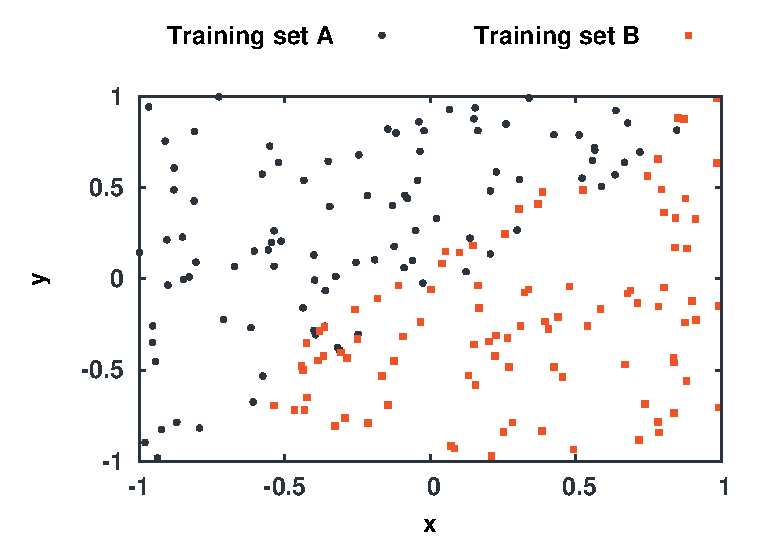
\includegraphics[width=0.48\textwidth]{figures/knn_95_55_separable_overlapped_weighted_samples.eps} \label{fig: knnSepTrainSetOvr}}
\hfill
\caption{Training sets for points separable by $f(x) = x$.}
\label{fig: knnSepTrainSet}
\end{figure}

Lets consider something defined mathematically better than {\it blue} and {\it orange}, i.e. two classes of points which can be separated linearly, e.g. by the line $f(x) = x$ as presented on Fig. \ref{fig: knnSepTrainSet} in three scenarios:

\begin{itemize}
 \item points are exactly separated by $f(x) = x$, Fig. \ref{fig: knnSepTrainSetDef}
 \item there is a small gap to make points more separated, Fig. \ref{fig: knnSepTrainSetDis}
 \item points overlap a little, Fig. \ref{fig: knnSepTrainSetOvr}
\end{itemize}

For each scenario the efficiency of kNN as a function of the size of training sets ($n$) and $k$ is checked in the following way:

\begin{enumerate}
 \item generate $n$ random points above $f(x) = x$ (training set A)
 \item generate $n$ random points below $f(x) = x$ (training set B)
 \item generate a random point
 \item find $k$ nearest neighbors of this point
 \item let them vote:
 \begin{itemize}
  \item with vote weight = $1$ (unweighted)
  \item with vote weight = $1/$distance (weighted)
 \end{itemize}
 \item repeat points 3-5 $N$ times to get good enough statistics ($N = 10^5$ for presented results, but every $100$ test points new training sets are generated)
 \item calculate the score = no. of correctly guessed points / no. of all test points
\end{enumerate}

The efficiency of kNN as a function of $k$ and $n$ can be found on Fig. \ref{fig: knnSepRes}. Clearly, weighted voting gives better results, especially for $k \sim n$. However, even unweighted kNN still gives score better than 90\%. The efficiency is almost the same when extra gap is generated between training sets (Figs. \ref{fig: knnSepResDisU} and \ref{fig: knnSepResDisW}), but it becomes much worse if training sets overlap (Figs. \ref{fig: knnSepResOvrU} and \ref{fig: knnSepResOvrW}).

\begin{figure}
\hfill
\subfigure[Default, unweighted]{\includegraphics[width=0.48\textwidth]{figures/knn_separable_default_unweighted.eps} \label{fig: knnSepResDefU}}
\hfill
\subfigure[Default, weighted]{\includegraphics[width=0.48\textwidth]{figures/knn_separable_default_weighted.eps} \label{fig: knnSepResDefW}}
\hfill
\subfigure[Distant, unweighted]{\includegraphics[width=0.48\textwidth]{figures/knn_separable_distant_unweighted.eps} \label{fig: knnSepResDisU}}
\hfill
\subfigure[Distant, weighted]{\includegraphics[width=0.48\textwidth]{figures/knn_separable_distant_weighted.eps} \label{fig: knnSepResDisW}}
\hfill
\subfigure[Overlapped, unweighted]{\includegraphics[width=0.48\textwidth]{figures/knn_separable_overlapped_unweighted.eps} \label{fig: knnSepResOvrU}}
\hfill
\subfigure[Overlapped, weighted]{\includegraphics[width=0.48\textwidth]{figures/knn_separable_overlapped_weighted.eps} \label{fig: knnSepResOvrW}}
\hfill
\caption{kNN efficiency for points separable by $f(x) = x$.}
\label{fig: knnSepRes}
\end{figure}

\begin{figure}
\hfill
\subfigure[Training sets]{\includegraphics[width=0.48\textwidth]{figures/knnWrongTrainSet.eps} \label{fig: knnWrongTrainSet}}
\hfill
\subfigure[Testing set]{\includegraphics[width=0.48\textwidth]{figures/knnWrongTrainResults.eps} \label{fig: knnWrongTrainResults}}
\hfill
\hfill
\caption{The example of the kNN classification using wrong training sets ($n = 100$, $k = 50$).}
\label{fig: knnWrongTrain}
\end{figure}

Lets take a look what happens when training sets are not uniformly distributed, as presented on Fig. \ref{fig: knnWrongTrain}. It still looks (by eye) that training sets are separated by $f(x) = x$, see Fig. \ref{fig: knnWrongTrainSet}. However, from obvious reasons some points are going to be incorrectly classified, as presented on Fig. \ref{fig: knnWrongTrainResults}.


\subsection{Inseparable points}
\label{sec: knnInSep}

\begin{figure}
\hfill
\subfigure[Default]{\includegraphics[width=0.48\textwidth]{figures/knn_95_55_inseparable_default_weighted_samples.eps} \label{fig: knnInSepTrainSetDef}}
\hfill
\subfigure[Distant]{\includegraphics[width=0.48\textwidth]{figures/knn_95_55_inseparable_distant_weighted_samples.eps} \label{fig: knnInSepTrainSetDis}}
\hfill
\centering\subfigure[Overlapped]{\includegraphics[width=0.48\textwidth]{figures/knn_95_55_inseparable_overlapped_weighted_samples.eps} \label{fig: knnInSepTrainSetOvr}}
\hfill
\caption{Training sets for inseparable points (inside / outside a circle).}
\label{fig: knnInSepTrainSet}
\end{figure}

Lets now consider points which are not linearly separable, i.e. points inside and outside a circle, as presented on Fig. \ref{fig: knnInSepTrainSet}. Once again, three cases are investigated: default (points exactly separated by a circle, Fig. \ref{fig: knnInSepTrainSetDef}), distant (with extra gap between training sets, Fig. \ref{fig: knnInSepTrainSetDis}), and overlapped (training sets are allowed to overlap a little, Fig. \ref{fig: knnInSepTrainSetOvr}).

\begin{figure}
\hfill
\subfigure[Default, unweighted]{\includegraphics[width=0.48\textwidth]{figures/knn_inseparable_default_unweighted.eps} \label{fig: knnInSepResDefU}}
\hfill
\subfigure[Default, weighted]{\includegraphics[width=0.48\textwidth]{figures/knn_inseparable_default_weighted.eps} \label{fig: knnInSepResDefW}}
\hfill
\subfigure[Distant, unweighted]{\includegraphics[width=0.48\textwidth]{figures/knn_inseparable_distant_unweighted.eps} \label{fig: knnInSepResDisU}}
\hfill
\subfigure[Distant, weighted]{\includegraphics[width=0.48\textwidth]{figures/knn_inseparable_distant_weighted.eps} \label{fig: knnInSepResDisW}}
\hfill
\subfigure[Overlapped, unweighted]{\includegraphics[width=0.48\textwidth]{figures/knn_inseparable_overlapped_unweighted.eps} \label{fig: knnInSepResOvrU}}
\hfill
\subfigure[Overlapped, weighted]{\includegraphics[width=0.48\textwidth]{figures/knn_inseparable_overlapped_weighted.eps} \label{fig: knnInSepResOvrW}}
\hfill
\caption{kNN efficiency for inseparable points.}
\label{fig: knnInSepRes}
\end{figure}

The efficiency, presented on Fig. \ref{fig: knnInSepRes}, is calculated exactly the same way as in Sec. \ref{sec: knnSep}. Please note the different scale which now starts at $0.4$. Clearly, unweighted kNN requires now larger training sets to get an efficiency $\geq 90\%$. It is expected, though. The more complex problem the larger training set is necessary. Weighted kNN still works (surprisingly?) pretty well even for small training sets.

\section{Support Vector Machine}
\label{sec: svm}

Support Vector Machine is one those algorithms which sounds pretty easy until you actually start using it. It is a binary classifier, so it can only work with two classes at a time. It is an extension of perceptron algorithm (sometimes known as perceptron with optimal stability). 

The perceptron algorithm looks for a line (or a hyperplane in general) which separates training sets. Thus, it works only for linearly separable classes. The hyperplane is found using online learning, by updating the hyperplane based on incorrectly classified training points. For linearly separable classes it guarantees convergence, but it does not control the final orientation of the hyperplane. As presented on Fig. \ref{fig: perceptron}, there is infinitely many hyperplanes (lines) like that.

\begin{figure}
  \centering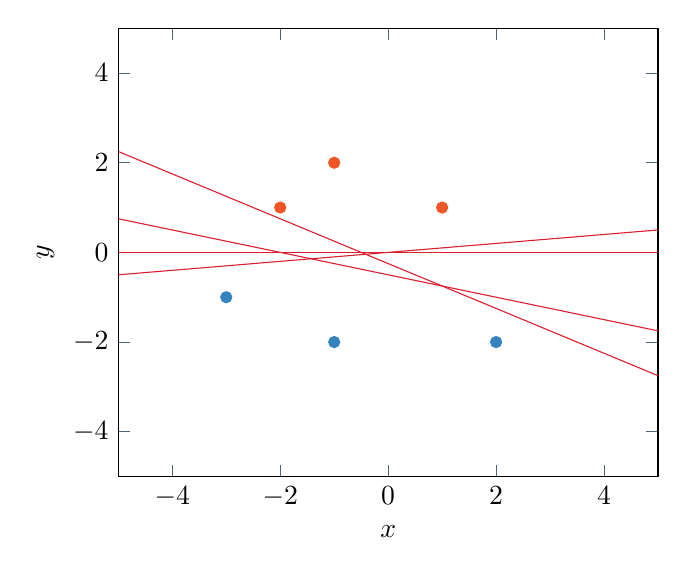
\begin{tikzpicture}

  \begin{axis}[xlabel = $x$, ylabel = $y$, xmin = -5.0, xmax = 5.0, ymin = -5.0, ymax = 5.0]
    
    \addplot[mark = *, , draw = none, color = orange] coordinates {(1,1)}; 
    \addplot[mark = *, , draw = none, color = orange] coordinates {(-1,2)}; 
    \addplot[mark = *, , draw = none, color = orange] coordinates {(-2,1)}; 

    \addplot[mark = *, , draw = none, color = blue] coordinates {(-1,-2)}; 
    \addplot[mark = *, , draw = none, color = blue] coordinates {(2,-2)}; 
    \addplot[mark = *, , draw = none, color = blue] coordinates {(-3,-1)}; 

    \addplot[color = red] {0};
    \addplot[color = red] {-0.25*x - 0.50};
    \addplot[color = red] {-0.50*x - 0.25};
    \addplot[color = red] {0.1*x};
    
    %\addplot[mark = *, , draw = none, color = red] coordinates {(-1,-1)};

  \end{axis}

\end{tikzpicture}
  \caption{Examples of separation lines for two-dimensional data.}
  \label{fig: perceptron}
\end{figure}

One can expect that the best separation hyperplane should be possible as far as possible from both testing samples. Intuitively, the ``real'' boundary separating classes (which is unknown) is located far from the center of training sets. This way, one may expect better classification of unusual testing points, so better generalization of the problem.

SVM guarantees (for linearly separable classes) finding the maximum-margin hyperplane. It can be easily extend for ``almost'' linearly separable classes, like those presented on Fig. \ref{fig: knnSepTrainSetOvr} (see Sec. \ref{sec: svmAlmost}). For classes linearly inseparable, {\it kernel trick} is used to transform feature space to higher dimension, where classes are linearly separable and maximum-margin hyperplane can be found (see Sec. \ref{sec: svmKernel}).

The task is ``easy'' - find the separation hyperplane and classification is straightforward.
\subsection{Linear SVM}
\label{fig: svmLinear}

Lets consider our training sets are given by:

\begin{equation}
  \left\{\left(\vec x_i, y_i\right)\right\}_{i=1,...,N}
  \label{eq: trainSet}
\end{equation}

where $\vec x_i = \left(x_{i1}, ... , x_{in}\right) \in \mathbb{R}^n$ are features vector in $n$-dimensional space, $y_i \in \left\{-1, 1\right\}$ defines membership to given class\footnote{$\left\{-1, 1\right\}$ was chosen for convenience in further calculations.}, $N$ is the size of training sets. A hyperplane can be defined by its normal vector ($\vec\omega = (\omega_1, ... , \omega_n)$) and an absolute term ($\omega_0$):

\begin{equation}
 \omega_0 + \underbrace{\omega_1 \cdot x_1 + ... + \omega_n\cdot x_n}_{\left<\vec\omega, \vec x\right>} = 0
 \label{eq: hyperplane}
\end{equation}

The distance ($d$) between a point $\vec x$ and a hyperplane defined by $\vec\omega$ and $\omega_0$ is given by the following formula:

\begin{equation}
 d \left(\vec x, \vec\omega, \omega_0\right) = \frac{\left|\omega_0 + \left<\vec\omega, \vec x\right>\right|}{||\vec\omega||}
 \label{eq: distance}
\end{equation}

where $||\vec\omega|| = \sqrt{\omega_1^2 + ... + \omega_n^2}$ is norm of the vector $\vec\omega$. Having that, the margin of separation ($\tau$) for training set from Eq. \ref{eq: trainSet} and a hyperplane as in Eq. \ref{eq: hyperplane} is defined as:

\begin{equation}
 \tau (\vec\omega, \omega_0) = \min_{i=1,...,N} \frac{y_i\cdot\left(\omega_0 + \left<\vec\omega, \vec x_i\right>\right)}{||\vec\omega||}
\end{equation}

so it is a distance between the hyperplane and the closest point. One should note, that absolute value from Eq. \ref{eq: distance} disappears because of smart choice of $y$ values. Points on the ``positive'' side of the hyperplane have $y = 1$, and those on the ``negative'' side have $y = -1$, which guarantees $\tau \geq 0$ (assuming all testing points are classified correctly).

\begin{figure}
 \centering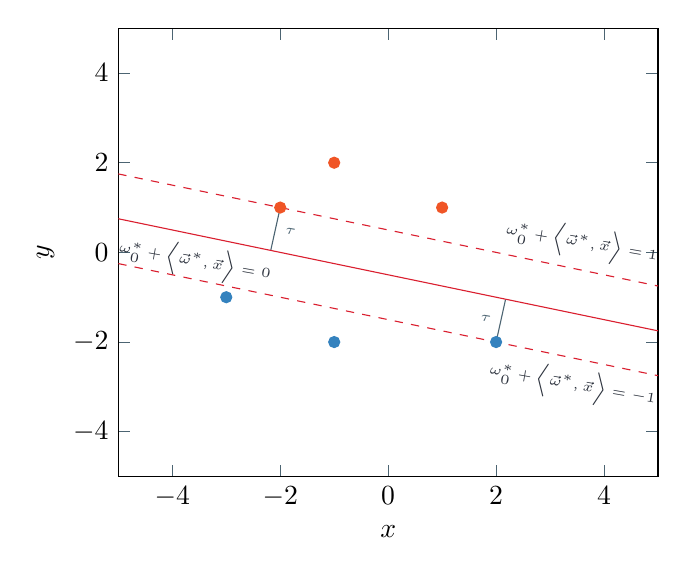
\begin{tikzpicture}

  \begin{axis}[xlabel = $x$, ylabel = $y$, xmin = -5.0, xmax = 5.0, ymin = -5.0, ymax = 5.0]
    
    \addplot[mark = *, , draw = none, color = orange] coordinates {(1,1)}; 
    \addplot[mark = *, , draw = none, color = orange] coordinates {(-1,2)}; 
    \addplot[mark = *, , draw = none, color = orange] coordinates {(-2,1)}; 

    \addplot[mark = *, , draw = none, color = blue] coordinates {(-1,-2)}; 
    \addplot[mark = *, , draw = none, color = blue] coordinates {(2,-2)}; 
    \addplot[mark = *, , draw = none, color = blue] coordinates {(-3,-1)}; 

    \addplot[mark = none, color = gray] coordinates {(-2,1) (-2.175,0.05)} node[right, pos=0.5, rotate=-10] {\tiny$\tau$}; 
    \addplot[mark = none, color = gray] coordinates {(2,-2) (2.175,-1.05)} node[left, pos=0.5, rotate=-10] {\tiny$\tau$}; 

    \addplot[color = red]         {-0.25*x - 0.5} node[below, pos=0.15, rotate=-10] {\color{black}\tiny$\omega_0^* + \left<\vec\omega^*, \vec x\right> = 0$};;
    \addplot[color = red, dashed] {-0.25*x - 1.5} node[below, pos=0.85, rotate=-10] {\color{black}\tiny$\omega_0^* + \left<\vec\omega^*, \vec x\right> = -1$};
    \addplot[color = red, dashed] {-0.25*x + 0.5} node[above, pos=0.85, rotate=-10] {\color{black}\tiny$\omega_0^* + \left<\vec\omega^*, \vec x\right> = 1$};;
    
  \end{axis}

\end{tikzpicture}
 \caption{The example of maximum-margin hyperplane separating two training sets. {\it Note, it is just a demonstrative cartoon, not real calculations.}}
 \label{fig: svmMargin}
\end{figure}

SVM is looking for the optimal hyperplane, so the one with the maximum margin of separation. The optimization task to solve is:

\begin{subequations}
 \begin{equation}
  \text{maximize}\hspace{10pt}\tau (\vec\omega, \omega_0)
 \end{equation}
 \begin{equation}
  \text{subject to}\hspace{10pt}\forall_i\hspace{5pt} y_i \cdot \left(\omega_0 + \left<\vec\omega, \vec x_i\right>\right) \geq \tau(\vec\omega, \omega_0)\cdot ||\vec\omega||
 \end{equation}
 \label{eq: optimization0}
\end{subequations}

Thus, maximize $\tau$ and make sure all points are on the right side of the hyperplane (with the distance not smaller than $\tau$). Please note, that there are still infinitively many hyperplanes fulfill these conditions (as multiplying Eq. \ref{eq: hyperplane} by a constant does not change the position of the hyperplane). One can use an arbitrary bond to determine the hyperplane unambiguously. It is convenient to use the following bond:

\begin{equation}
 \tau(\vec\omega, \omega_0)\cdot ||\vec\omega|| = 1
\end{equation}

With this bond, maximizing $\tau$ can be considered as minimizing the length of normal vector $||\vec\omega||$, so the optimization conditions from Eq. \ref{eq: optimization0} can be rewritten as:

\begin{subequations}
 \begin{equation}
  \text{minimize}\hspace{10pt} Q(\vec\omega) = \frac{1}{2}||\vec\omega||^2
  \label{eq: maximize}
 \end{equation}
 \begin{equation}
  \text{subject to}\hspace{10pt}\forall_i\hspace{5pt} y_i \cdot \left(\omega_0 + \left<\vec\omega, \vec x_i\right>\right) \geq 1
  \label{eq: condition}
 \end{equation}
 \label{eq: optimization}
\end{subequations}

where $\frac{1}{2}$ in Eq. \ref{eq: maximize} is just for convenience in further calculations. For the same reasons, the square of $||\vec\omega||$ is considered. It does not affect the final result as $||\vec\omega||$ and $Q(\vec\omega)$ have the minimum for the same $\vec\omega$. 

The example of maximum-margin hyperplane separating two training sets is presented on Fig. \ref{fig: svmMargin}, where $\omega_0^*$ and $\vec\omega^*$ denote the solution of Eq. \ref{eq: optimization}. Please note, this is just a demonstrative cartoon, not a real solution.

Eq. \ref{eq: optimization} is a quadratic programming problem. It is a kind of mathematical optimization which is extensively studied. There are many methods to solve this kind of problems. In the context of SVM Lagrange multipliers is commonly used. Sec. \ref{sec: lm} is an introduction / reminder on Lagrange multipliers. In Sec. \ref{sec: svmLinearLM} Eq. \ref{eq: optimization} is solved using this method.

\end{document}
